\chapter{Introduction}
\label{sec:test}

This is a template made for PhD dissertations at The Hong Kong Polytechnic University, and follows the university's requirements stipulated in the Research Postgraduate Student Handbook (\url{https://www.polyu.edu.hk/gs/rpghandbook/ref-regulations-format-thesis}). The original of this \hologo{LaTeX} template was created by \href{https://github.com/ragonneau}{Tom M. Ragonneau}, at the Department of Applied Mathematics (you can access it here \url{https://github.com/ragonneau/phd-thesis-template}), and subsequently modified by \href{https://github.com/partigabor}{Gábor Parti}, Department of Chinese and Bilingual Studies. This version is tailored for linguistics-oriented theses, and supports multi-scripted documents. It is optimized for \hologo{LuaLaTeX}.

A thesis submitted for examination purpose should include the words ‘Initial Submission for Examination Purpose’ lettered on the front cover.

\section{Typesetting}
\subsection{Typesetting}
\subsubsection{Typesetting}
\marginpar{A `subsubsection' will not appear in the ToC... }

\lettrine[lines=5, slope=0.5em, lraise=0, nindent=1em, findent=-1em]{\textcolor{\accentcolor}{A}} nearly full list of features and tools are tested here, from typesetting to citations. \blindtext

\medskip 

Normal, \textit{italic}, \textbf{bold}, \textbf{\textit{bold-italic}}, UPPERCASE,\textsc{small-capitals}\footnote{If you don't see \emph{small capitals}, your font does not have them.}, \textss{superscript}, \hl{highlight}.

\medskip

1234567890 \nth{1} \nth{2} \nth{3} \nth{4} \nth{19} \BC{} \AD{} . , : ; ? ! ``'' \$ \& \% \# () [] \{\} \textbackslash / <> || - -- --- + = *

\medskip

Ligatures --- Common: ff, fi, and ffi; Rare: st, ct, is.

\begin{table}[ht]
    \caption{Different font styles and typefaces.}
\begin{tabular}{@{}lll@{}}
\toprule
Normal      & Sphinx of black quartz, judge my missing vow forever. \\
Italic      & \textit{Sphinx of black quartz, judge my missing vow forever.} \\
Bold        & \textbf{Sphinx of black quartz, judge my missing vow forever.} \\
Bold-Italic & \textbf{\textit{Sphinx of black quartz, judge my missing vow forever.}} \\
Uppercase   & \uppercase{Sphinx of black quartz, judge my missing vow forever.} \\
Small caps  & \textsc{Sphinx of black quartz, judge my missing vow forever.} \\
Superscript & \textss{Sphinx of black quartz, judge my missing vow forever.} \\
Sans serif  & \textsf{Sphinx of black quartz, judge my missing vow forever.} \\
Mono        & \texttt{Sphinx of black quartz, judge my missing vow forever.} \\ \bottomrule
\end{tabular}
\end{table}

\noindent{\color{black}\rule{0.25\linewidth}{0.2mm}} this is baseline

\noindent{\color{black}\rule[0.5ex]{0.25\linewidth}{0.2mm}} this is half raised

\noindent{\color{black}\rule[1ex]{0.25\linewidth}{0.2mm}} this is raised

\noindent{\color{black}\rule[1.5ex]{0.25\linewidth}{0.2mm}} this is raised above

\section{Scripts}

Various scripts and languages:

Akkadian: \cu{𒀝𒅗𒁺𒌑}

Amharic: \am{አማርኛ}

Arabic: \ar{العربية}

Aramaic: \sy{ܠܫܢܐ ܣܘܪܝܝܐ}

Armenian: \hy{Արևելահայերեն}

% Balinese: 

% Bengali: বাংলা

Chinese, Traditional: 廣東話 \tc{漢語}

Chinese, Simplified: 汉语 \zh{汉语}

Coptic: \co{ⲘⲉⲧⲢⲉⲙ̀ⲛⲭⲏⲙⲓ}

Georgian: \ka{ქართული ენა}

Greek: Ελληνικά

Hebrew: \he{עברית}

Japanese: 日本語 にほんご ニホンゴ

Javanese: \jv{ꦧꦱꦗꦮ}

Korean: 한국어

Linear B: \lb{𐀏𐁁𐀪𐃠}

Macedonian: Македонски

Malayalam: \ml{മലയാളം}

% Mongolian: \mn{ᠬᠣᠭᠣᠷᠣᠨᠳᠣ᠎ᠨ}

Old South Arabian: \osa{𐩣𐩥𐩵𐩩𐩺𐩤𐩱𐩧𐩦𐩬}

Persian: \fa{فارسی}

% Punjabi: ਪੰਜਾਬੀ

Sanskrit: \sa{संस्कृतम्}

Tamil: \ta{தமிழ்}

Thai: \thai{ภาษาไทย}

Tibetan: \ti{བོད་སྐད་}

Urdu: \ur{اردو}

Vietnamese: tiếng việt

% % \textbf{Latin}: A a, Á á, B b, C c, Cs cs, D d, Dz dz, Dzs dzs, E e, É é, F f, G g, Gy gy, H h, I i, Í í, J j, K k, L l, Ly ly, M m, N n, Ny ny, O o, Ó ó, Ö ö, Ő ő, P p, Q q, R r, S s, Sz sz, T t, Ty ty, U u, Ú ú, Ü ü, Ű ű, V v, W w, X x, Y y, Z z, Zs zs.

% % \textbf{Greek}: Α α, Β β, Γ γ, Δ δ, Ε ε, Ζ ζ, Η η, Θ θ, Ι ι, Κ κ, Λ λ, Μ μ, Ν ν, Ξ ξ, Ο ο, Π π, Ρ ρ, Σ σ/ς, Τ τ, Υ υ, Φ φ, Χ χ, Ψ ψ, Ω ω.

% % \textbf{Cyrillic}: A a, Б б, В в, Г г, Д д, Ѓ ѓ, E e, Ж ж, З з, Ѕ ѕ, И и, J j, К к, Л л, Љ љ, М м, Н н, Њ њ, О о, П п, Р р, С с, Т т, Ќ ќ, У у, Ф ф, Х х, Ц ц, Ч ч, Џ џ, Ш ш.

\subsubsection{Bidirectional Scripts}

Arabic and Hebrew in English paragraphs, in mixed environments:

ما هو \foreignlanguage{english}{differentiation}? 

What is ما هو in Arabic?
\medskip
\textnormal
\noindent Most Arabic speakers consider the two varieties to be two registers
of one language, although the two registers can be referred to in
Arabic as فصحى العصر \textit{fuṣḥā l-ʻaṣr} Modern Standard Arabic (MSA) and
فصحى التراث \textit{fuṣḥā t-turāth} Classical Arabic (CA). ʿArab\={i}.

\medskip

The first line of the Bible is בְּרֵאשִׁית בָּרָא אֱלֹהִים אֵת הַשָּׁמַיִם וְאֵת הָאָרֶץ (Genesis 1:1).

% % Actual right-to-left paragraphs (warning).
% \selectlanguage{arabic}
% مكانة عائلته الاجتماعية مكنته من الدراسة على يد أفضل المدرسين في المغرب العربي. تلقى علم التربية الإسلامية التقليدية، ودرس القرآن الكريم الذي كان يحفظه عن ظهر قلب، واللسانيات العربية، وأساس فهم القرآن، الحديث، الشريعة (القانون) والفقه علم التاريخ.
% \selectlanguage{english}

% For inline usage: \foreignlanguage{hebrew}{תַּבְלִין}

\section{Acronyms, Glossary Terms, and Indexing}

The \hologo{LaTeX} typesetting markup language is specially suitable for documents that are annoying to make.

\bigskip

Glossaries and acronyms both have to be set in the glossary.tex with similar methods, and then called in the text. When an acronym appears for the first time, its full form is also shown. Such as, \gls{OED} but the second time \gls{OED}. For plural and capital glossaries use \gls{taxon} and \glspl{taxon}; \Gls{taxon} and \Glspl{taxon}.

Index one\index{one} is here and \index{other one} two\index{two} is here. There is also index for tables \index{three|tb}, figures\index{four|fg}, and footnotes\index{five|fn}.
Also, there is grouped indexing possible for things like black pepper\index{pepper!black}, white pepper\index{pepper!white}, and green pepper\index{pepper!green}. 

% WARNING: The index on Overleaf only prints on your pdf if you run it for the first time/clear the cache. I don't know why, currently unsolved.

\section{Citations}

Citation examples, such as \autocite[99]{laufer_sino-iranica_1919}, which now is the same as \parencite[99]{laufer_sino-iranica_1919} and \textcite{laufer_sino-iranica_1919}, but footcite also exists.\footcite{laufer_sino-iranica_1919} 
Multi-volume citing is also available, \pvolcite[]{9}[99]{ei2} \& \tvolcite[]{9}[99]{ei2}.

\section{Lists and Environments}
\label{sec:environments}

\begin{enumerate}
    \item one
    \item two
    \item three
\end{enumerate}

\begin{itemize}
    \item one
    \item two
    \item three
\end{itemize}

\begin{note}
    This is a note.
\end{note}

\begin{equation}
    \label{eq:1}
    x^2  = 1
\end{equation}

This (above) is an equation. In Equation \ref{eq:1} we have~$\sqrt{\log n}$.

\ex
\begingl
\gla\rightcomment{Hungarian (Finno-Ugric, \emph{reference})}Ez egy nyelvészeti példamondat.//
\glb This a linguistic example-sentence//
\glft ``This is a linguistic example sentence.''//
\endgl
\xe

\begin{etymology}\label{etym:pepper}
\raggedright
English \textit{pepper}
< Middle English \textit{peper}
< Old English \textit{pipor}
< West Germanic \textit{*piper}
< Latin \textit{piper} `black pepper, long pepper'
< Ancient Greek \textit{péperi} `pepper'
< Pahlavi
< Middle Indo-Aryan \textit{pipparī} `long pepper'
< Sanskrit \textit{pippalī} `berry, peppercorn', \textit{pippali} `long pepper'\footnote{This is a custom, iterating environment that you can modify for whatever purpose.}
\end{etymology}

This line has a reference for Etymology \ref{etym:pepper} and a `clever reference' for \Cref{sec:environments}. And below is a quote.

\epigraph{By convention sweet and by convention bitter, by convention hot, by convention cold, by convention color; but in reality atoms and void.}{Democritus, \nth{3} century BC\\(DK 68B9, trans. Taylor 1999a)}

\section{Figures}

\begin{figure}[ht]
    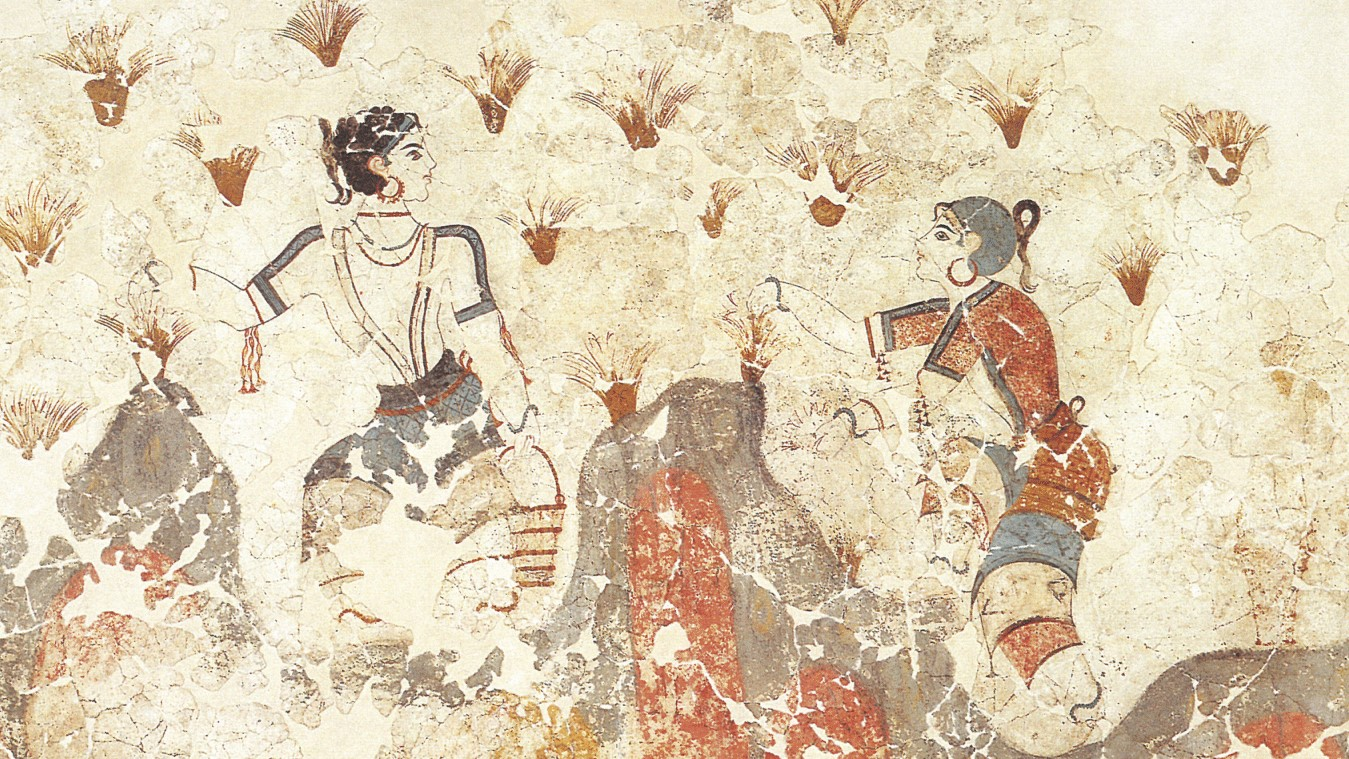
\includegraphics[width=\linewidth]{imgs/saffron_gatherers.jpg}
    \caption[Short caption to ToC]{Long caption}
    \label{fig:saffron1}
\end{figure}

\todo{Place figures better}

\begin{figure}[!hbt]
    \centering
    \subfloat{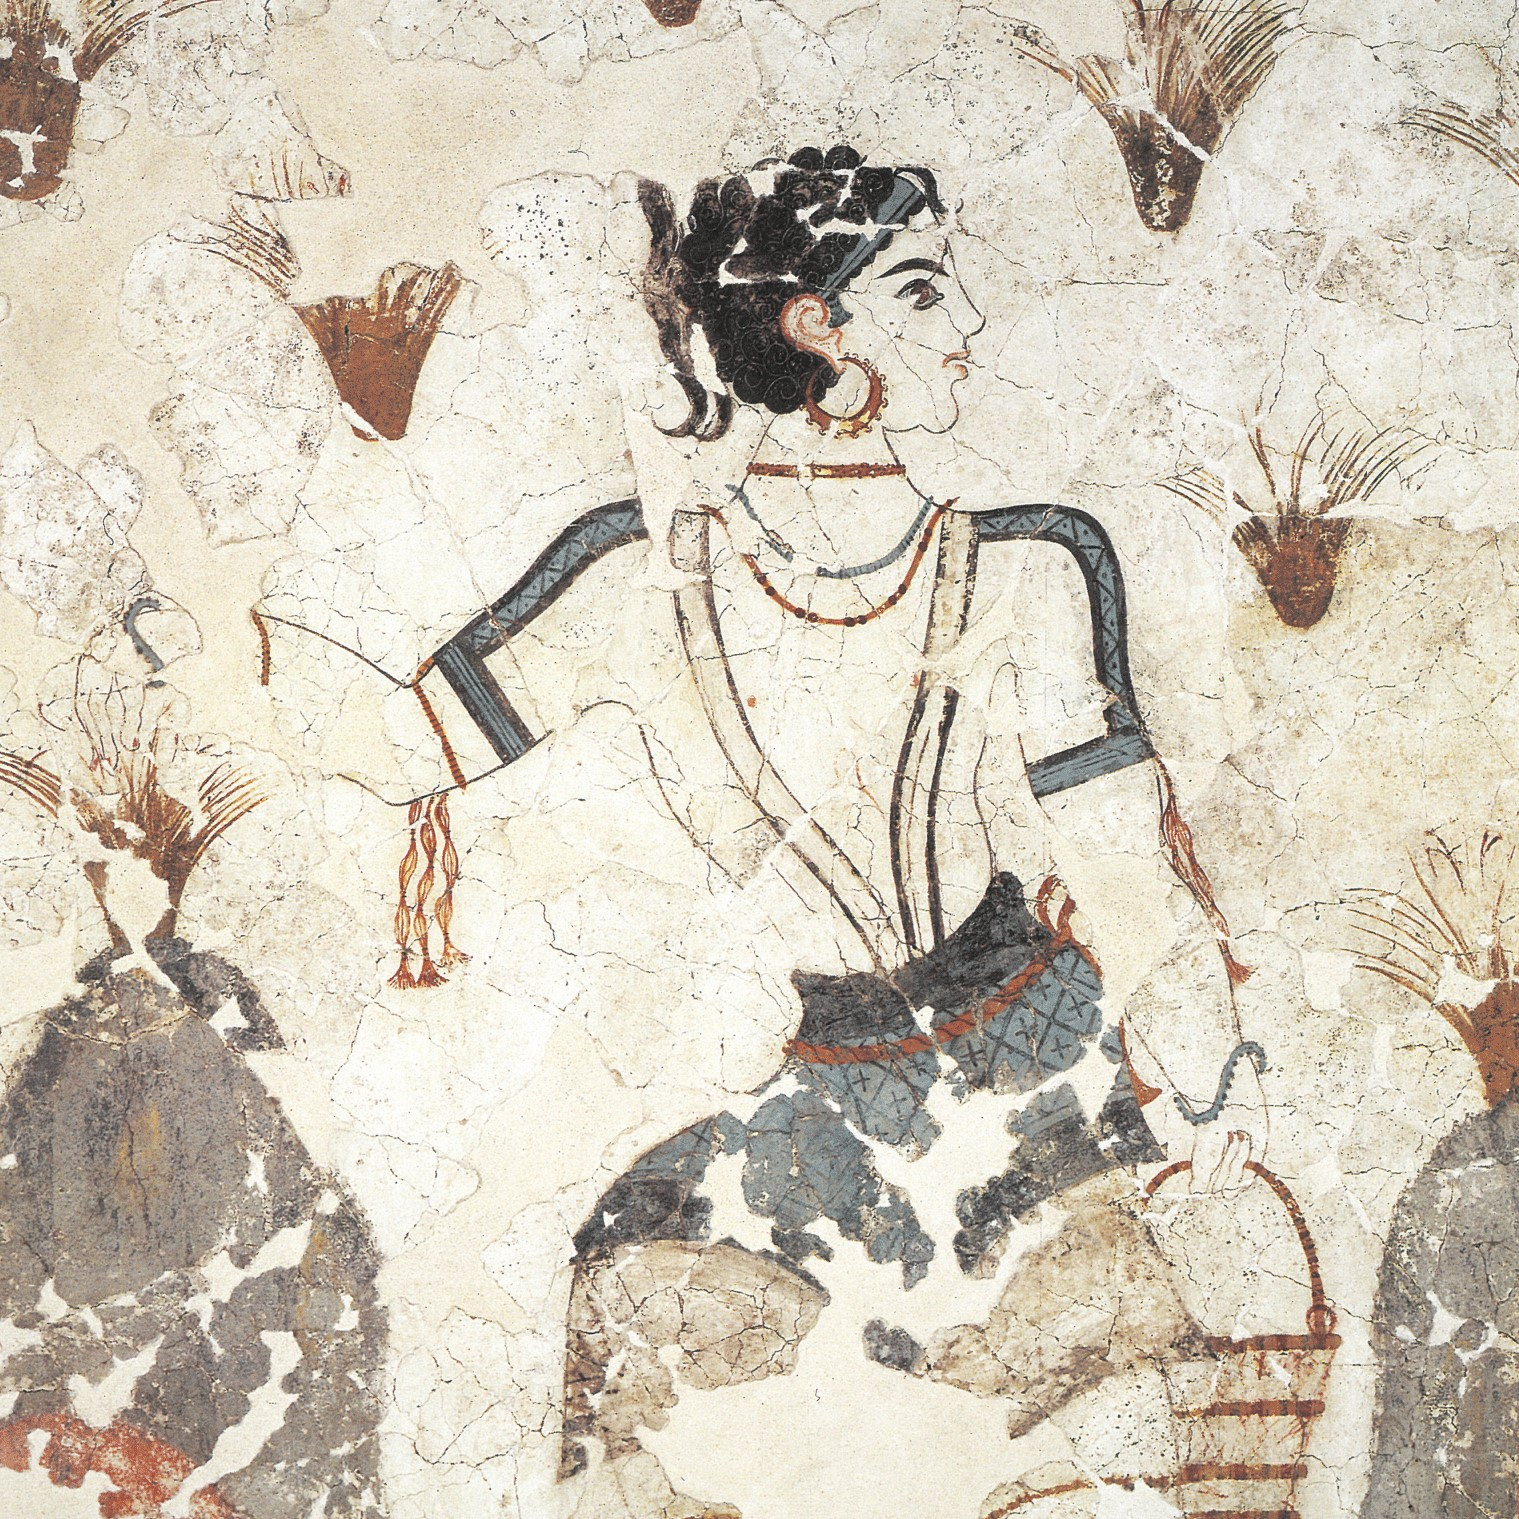
\includegraphics[width=0.482\linewidth]{imgs/saffron_gatherers_l.jpg}}
    \hfill
    \subfloat{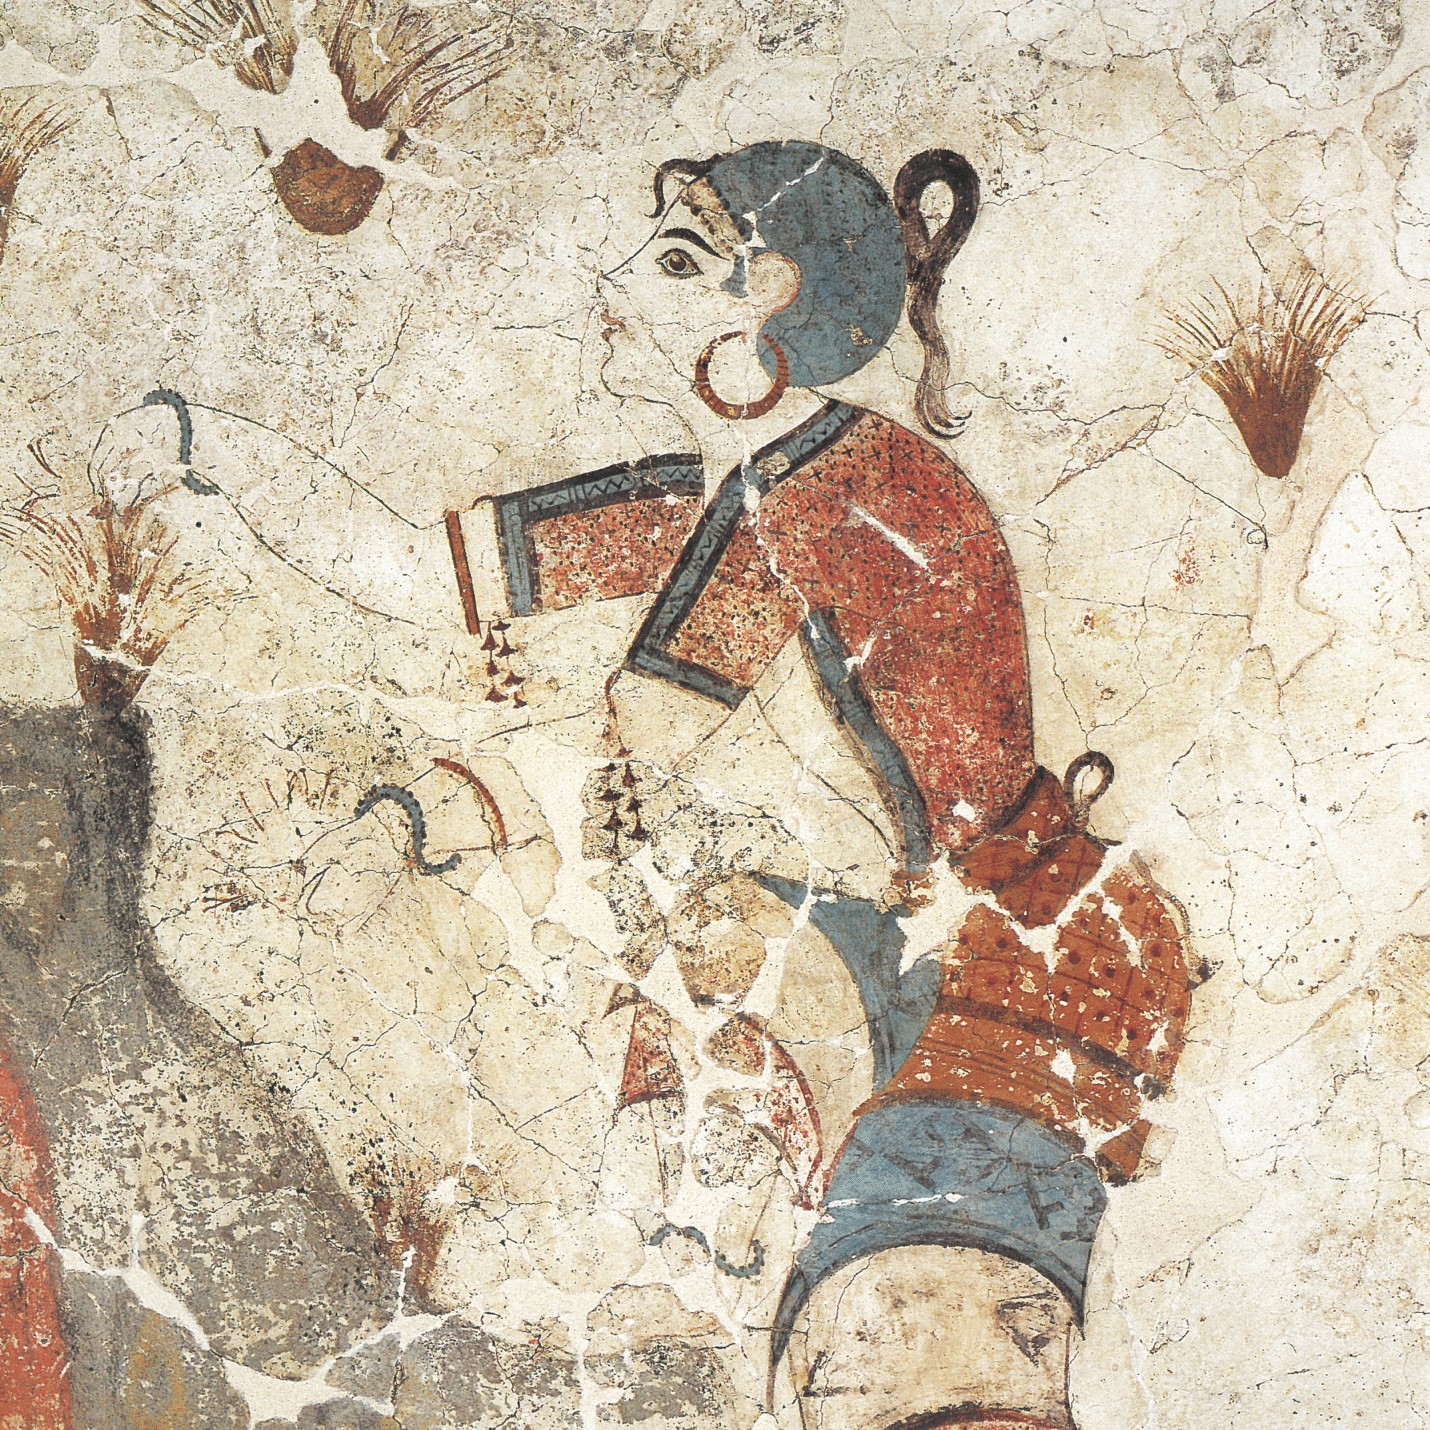
\includegraphics[width=0.482\linewidth]{imgs/saffron_gatherers_r.jpg}}
    \caption[Saffron-gatherers]{Saffron-gatherers; details from the mural on the east wall in room 3a, first floor, at Xeste 3 site, Akrotiri at Thera \autocite[152]{doumas_wall-paintings_1992}.}
    \label{fig:saffron2}
\end{figure}

\blindtext

\section{Trees}

\begin{center}
\begin{forest}
    for tree={align=center}
    [paprika\\\small{English}
    [paprika\\\small{Hungarian} 
    [pàprika\\\small{Serbian-Croatian-Bosnian} 
    [*pĭpĭrĭ\\\small{Proto-Slavic} 
    [piper\\\small{Latin} 
    [péperi\\\small{Ancient Greek},name=AG 
    [*\\\small{Pahlavi} 
    [pipparī\\\small{Middle Indo-Aryan} 
    [pippalī\\\small{Sanskrit}]]]]]] 
    [piperi\\\small{Modern Greek},edge=dashed,name=MG]]]]
    \draw[-] (AG.north) to (MG.south);
    \draw[->,dotted] (AG) to[out=east,in=south] (MG);
\end{forest}
\begin{tabular}[t]{ll@{}}
\tikz[baseline]\draw(0,1ex)--(1,1ex); & borrowed\\
\tikz[baseline]\draw[dotted](0,1ex)--(1,1ex); & descended\\
\tikz[baseline]\draw[dashed](0,1ex)--(1,1ex); & influenced\\
\end{tabular}
\end{center}

\blindtext


\section{Tables}

\setlength{\tabcolsep}{3pt} % Change separator length

\begin{table}[ht]
    \caption[An elaborate table]{The set of 24 spices included in this thesis, with scientific names of the source plant, names in English, Chinese, Arabic, and their transliterations.}
% \begin{adjustbox}{max width=\textwidth}
\begin{tabularx}{\textwidth}{@{}r>{\footnotesize}llll@{}rl@{}}
\toprule
\textbf{\#} & \multicolumn{1}{l}{\textbf{Species}} & \textbf{English} & \textbf{Chinese} & \textbf{Translit.} & \textbf{Arabic} & \textbf{Translit.}     \\ \midrule
1           & \textit{Pimenta dioica}            & allspice         & 多香果              & \textit{duōxiāngguǒ}     & فلفل إفرنجي     & \textit{filfil ifranjī}      \\
2           & \textit{Pimpinella anisum}         & anise            & 茴芹               & \textit{huíqín}          & ينسون           & \textit{yansūn}              \\
3           & \textit{Ferula assa-foetida} et al.& asafoetida       & 阿魏               & \textit{āwèi}            & حلتیت           & \textit{ḥiltīt}              \\
4           & \textit{Carum carvi}               & caraway          & 葛縷子              & \textit{gělǚzi}          & كراويا          & \textit{karāwiyā}            \\
5           & \textit{Elettaria cardamomum}      & cardamom         & \tc{荳蔻}            & \textit{dòukòu}          & هال             & \textit{hāl}                 \\
6           & \textit{Cinnamomum cassia}         & cassia           & 肉桂               & \textit{ròuguì}          & سليخة           & \textit{salīkha}             \\
7           & \textit{Capsicum annuum} et al.    & chile            & 辣椒               & \textit{làjiāo}          & فلفل حار        & \textit{fulful hārr}         \\
8           & \textit{Cinnamomum verum}          & cinnamon         & 錫蘭肉桂             & \textit{xīlánròuguì}     & قرفة            & \textit{qirfa}               \\
9           & \textit{Syzygium aromaticum}       & clove            & 丁香               & \textit{dīngxiāng}       & قرنفل           & \textit{qaranful}            \\
10          & \textit{Coriandrum sativum}        & coriander        & \tc{芫荽}               & \textit{yánsui}          & كزبرة           & \textit{kuzbara}             \\
11          & \textit{Cuminum cyminum}           & cumin            & 孜然               & \textit{zīrán}           & كمون            & \textit{kammūn}              \\
12          & \textit{Anethum graveolens}        & dill             & 蒔蘿               & \textit{shíluó}          & شبت             & \textit{shibitt}             \\
13          & \textit{Foeniculum vulgare}        & fennel           & 茴香               & \textit{huíxiāng}        & شمر             & \textit{shamar}              \\
14          & \textit{Trigonella foenum-graecum} & fenugreek        & 胡蘆巴              & \textit{húlúbā}          & حلبة            & \textit{ḥulba}               \\
15          & \textit{Zingiber officinale}       & ginger           & 薑                & \textit{jiāng}           & زنجبيل          & \textit{zanjabīl}            \\
16          & \textit{Piper longum}              & long pepper      & 蓽撥               & \textit{bìbō}            & دار فلفل        & \textit{dār filfil}          \\
17          & \textit{Myristica fragrans}        & mace             & \tc{肉荳蔻皮}             & \textit{ròudòukòupí}    & بسباسة	& \textit{basbāsa} \\
18          & \textit{Myristica fragrans}        & nutmeg           & \tc{肉荳蔻}          & \textit{ròudòukòu}       & جوز الطيب       & \textit{jawz al-ṭīb}         \\
19          & \textit{Piper nigrum}              & pepper           & 胡椒               & \textit{hújiāo}          & فلفل            & \textit{filfil, fulful}      \\
20          & \textit{Crocus sativus}            & saffron          & 番紅花              & \textit{fānhónghuā}      & زعفران          & \textit{zaʿfarān}            \\
21          & \textit{Zanthoxylum spp.}          & Sichuan pepper   & 花椒               & \textit{huājiāo}         & فلفل سيتشوان    & \textit{filfil sītshuwān}    \\
22          & \textit{Illicium verum}            & star anise       & 八角               & \textit{bājiǎo}          & ينسون نجمي      & \textit{yansūn najmī}        \\
23          & \textit{Curcuma longa}             & turmeric         & 薑黃               & \textit{jiānghuáng}      & كركم            & \textit{kurkum}              \\
24          & \textit{Vanilla planifolia}        & vanilla          & 香草               & \textit{xiāngcǎo}        & فانيليا         & \textit{fānīliyā}\\ 
\midrule
 & & & & & & \\ \midrule
25          & \textit{Physeter macrocephalus*} & ambergris        & 龍涎香              & \textit{lóngxiánxiāng}   & عنبر            & \textit{ʿambar}          \\
26          & \textit{Cinnamomum camphora}     & camphor          & 樟                & \textit{zhāng}           & كافور           & \textit{kāfūr}           \\
27          & \textit{Moschus moschiferus*}    & musk             & 麝香               & \textit{shèxiāng}        & مسك             & \textit{misk}            \\
28          & \textit{Boswellia sacra}         & frankincense     & 乳香               & \textit{rǔxiāng}         & لبان            & \textit{lubān}           \\
29          & \textit{Commiphora myrrha}       & myrrh            & 沒藥               & \textit{mòyào}           & مر              & \textit{murr}            \\
30          & \textit{Santalum album}          & santalwood       & 旃檀               & \textit{zhāntán}         & الصندل          & \textit{ṣandal}          \\ 
\bottomrule
\end{tabularx}
% \end{adjustbox}
\label{table:set}
\end{table}

\setlength{\tabcolsep}{6pt} % Default separator length

\section{IPA}

\textipa{[ðIsIzsAmaIpeI]}, \textipa{[Its\*rilijizitutaIp]} as in: ``This is some IPA, it's really easy to type.''

\begin{longtable}{p{0.15\textwidth}p{0.3\textwidth}p{0.3\textwidth}}
  \toprule
  \endfirsthead
  \toprule
  \endhead
  \bottomrule
  \endfoot
  \bottomrule
  \endlastfoot
  Consonant & Onset & Coda\tabularnewline

  \midrule p & pun.za (claw) & \textipa{k\super hap.Ra} (old man)\tabularnewline

  b & \textipa{bO\|[d\super h} (bull) & \textipa{Seb.Ra} (dull)\tabularnewline

  \textipa{b\super h} & \textipa{b\super he\:d} (sheep) & \tabularnewline

  m & \textipa{mE} (me) & \textipa{amb} (mango)\tabularnewline

  f & ful (flower) & \tabularnewline

  \textipa{V} & \textipa{Vi\|[d.jaR.\|[t\super hi} & \textipa{RoVa}
  (injury)\tabularnewline

  \textipa{\|[t} & \textipa{\|[tu} (you) & \textipa{mO\|[t}
  (don't)\tabularnewline

  \textipa{\|[d} & \textipa{\|[deS} (many) & \textipa{swa\|[d}\tabularnewline

  \textipa{\|[t\super h} & \textipa{\|[t\super he\:n.\:di} (cold) &
  \textipa{hO\|[t\super h} (hand)\tabularnewline

  \textipa{\|[d\super h} & \textipa{\|[d\super hus.ki} (down) &
  \textipa{bO\|[d\super h} (bull)\tabularnewline

  \textipa{\t*{ts}} & \textipa{\t*{ts}Ol.\:na} (to walk) & \textipa{so\t*{ts}}
  (think)\tabularnewline

  \textipa{\t*{ts}\super h} & \textipa{\t*{ts}\super hekke} (fast) &
  \tabularnewline

  \textipa{\t*{dz}} & \textipa{\t*{dz}a.\:na} (to go) & \tabularnewline

  \textipa{n} & \textipa{n@i} (no) & \textipa{an.\|[dRe} (inside)\tabularnewline

  \textipa{R} & \textipa{me.Ri} (my) & \textipa{g\super hOR}\tabularnewline

  \textipa{s} & \textipa{sen.\|[tRi} (orange colour) & \textipa{hOs\:na} (to
  laugh)\tabularnewline

  \textipa{z} & \textipa{ze\:d} (root) & \textipa{Roz} (everyday)\tabularnewline

  \textipa{l} & \textipa{lOm.ma} (long) & \textipa{kal}
  (yesterday)\tabularnewline

  \textipa{S} & \textipa{Sob.la} (beautiful) & \textipa{gaS}
  (rain)\tabularnewline

  \textipa{\:t} & \textipa{\:te\:d.\:da} (curved) & \textipa{nO\:t.\:t\super he}
  (gone)\tabularnewline

  \textipa{\:t\super h} & \textipa{\:t\super he\:n\:ra} (cold) &
  \textipa{nO\:t.\:t\super he} (gone)\tabularnewline

  \textipa{\:d} & & \textipa{ne\:d} (near)\tabularnewline

  \textipa{\:d\super h} & & \textipa{pO\:d\super h.na} (to read)\tabularnewline

  \textipa{\:r} & \textipa{pO\:ru} (fell) & \textipa{me\:n.\:r\super h@k}
  (frog)\tabularnewline

  \textipa{\:n} & \textipa{\|[de.\:na} (to give) & \textipa{ku\:n}
  (who)\tabularnewline

  \textipa{\:l} & \textipa{ke\:la} (banana) & \tabularnewline

  \textipa{\t*{tS}} & \textipa{\t*{tS}Ok.ku\|[da} (rotten) & \tabularnewline

  \textipa{\t*{dZ}} & \textipa{\t*{dZ}epuR} (Jaipur) & \tabularnewline

  \textipa{j} & \textipa{ja\|[d} (remember) & \textipa{gaj}
  (abuse)\tabularnewline

  \textipa{k} & \textipa{ki.\:ra} (snake) & \textipa{b\super huk}
  (hunger)\tabularnewline

  \textipa{g} & \textipa{ga} (cow) & \textipa{b\super hEg.\:na} (to
  run)\tabularnewline

  \textipa{k\super h} & \textipa{k\super ha\:na} (to eat) & \textipa{paNk\super
    h} (wing)\tabularnewline

  \textipa{g\super h} & \textipa{g\super hOR} (house) & \tabularnewline

\end{longtable}































% \chapter{Testing}
% \label{sec:test}

% \lettrine[lines=4, lraise=0.1, nindent=0em, slope=-.5em]%
% {\textcolor{PolyU}{V}}{oici} un exemple... 

% \lettrine[lines=6, slope=0.5em, findent=-1em]%
% {A}{} nearly full list of features and tools are tested here, from typesetting to citations. 

% \blindtext[1]

% \bigskip



% 1234567890 .,:;?!@ \# \$ \% \^ \& \* () [] \{\} <> || - + = * ``Common'' ligatures ff, fi, and ffi, ``rare'' ones are st, ct, is. \textsc{smallcaps} and \textss{superscript}. \nth{1} \nth{2} \nth{3} \nth{4} \nth{19} century \BC{}, \AD{}. (if you don't see \emph{small capitals} \textsc{here}, the font does not have them).

% \noindent{\color{black}\rule{\linewidth}{0.2mm}} 

% \section{Section}

% \subsection{Subsection}

% \subsubsection{Subsubsection} 

% A `subsubsection' will not appear in the TOC. \marginpar{TOC means Table of Contents}


% \noindent{\color{black}\rule{0.25\linewidth}{0.2mm}} this is baseline

% \noindent{\color{black}\rule[0.5ex]{0.25\linewidth}{0.2mm}} this is half raised

% \noindent{\color{black}\rule[1ex]{0.25\linewidth}{0.2mm}} this is raised

% \noindent{\color{black}\rule[1.5ex]{0.25\linewidth}{0.2mm}} this is raised above

% \section{Typesetting}

% \begin{table}
% \begin{tabular}{@{}lll@{}}
% \toprule
% Normal      & Sphinx of black quartz, judge my missing vow forever. \\
% Bold        & \textbf{Sphinx of black quartz, judge my missing vow forever.} \\
% Italic      & \textit{Sphinx of black quartz, judge my missing vow forever.} \\
% Bold-Italic & \textbf{\textit{Sphinx of black quartz, judge my missing vow forever.}} \\
% Small caps  & \textsc{Sphinx of black quartz, judge my missing vow forever.} \\
% Uppercase   & \uppercase{Sphinx of black quartz, judge my missing vow for} \\
% Sans serif  & \textsf{Sphinx of black quartz, judge my missing vow forever.} \\
% Mono        & \texttt{Sphinx of black quartz, judge my missing vow forever.} \\ \bottomrule
% \end{tabular}
% \caption{Different font styles of the typeface.}
% \end{table}


% \bigskip

% Various scripts and languages:\marginpar{This is a marginpar, and it should go on the outer margin automatically.}

% Hungarian: köszönöm szépen \textit{köszönöm szépen} \textbf{köszönöm szépen}

% Greek: ευχαριστώ \textit{ευχαριστώ} \textbf{ευχαριστώ}

% Russian: спасибо \textit{спасибо} \textbf{спасибо}

% Chinese, Simplified: \zh{汉字:艹草,谢谢。 \textbf{汉字:艹草,谢谢。}}

% Chinese, Traditional: \tc{漢字:艸草,謝謝。 \textbf{漢字:艸草,謝謝。}}

% Chinese, Simplified: 汉字:艹草,谢谢。 \textbf{汉字:艹草,谢谢。}

% Chinese, Traditional: 漢字:艸草,謝謝。 \textbf{漢字:艸草,謝謝。}

% Japanese: ありがとうございました \textbf{ありがとうございました }

% Korean: 감사합니다 \textbf{감사합니다}

% \textnormal
% Devanagari: धन्यवाद \textbf{धन्यवाद}

% Arabic: شكرا جزيلا  \textit{شكرا جزيلا} \textbf{شكرا جزيلا}

% \textnormal
% Hebrew: תֹהוּ וָבֹהוּ \textbf{תֹהוּ וָבֹהוּ} 

% Tibetan: {\tibetanfont{ཐུགས་རྗེ་ཆེ་།} \textbf{ཐུགས་རྗེ་ཆེ་།}}

% Javanese: {\javanesefont{ꦩꦠꦸꦂꦤꦸꦮꦸꦤ꧀} \textbf{ꦩꦠꦸꦂꦤꦸꦮꦸꦤ꧀}}

% Tamil: {\tamilfont{மிக்க நன்றி} \textbf{மிக்க நன்றி}}

% Sumero-Akkadian Cuneform: {\cuneifont{\GA \NU \UU \UM \Leftarrow \GI}}


% \section{Bidirectional scritps}

% Arabic and Hebrew in English paragraphs, in mixed environments:

% ما هو \foreignlanguage{english}{differentiation}? 

% What is ما هو in Arabic?
% \medskip
% \textnormal
% \noindent Most Arabic speakers consider the two varieties to be two registers
% of one language, although the two registers can be referred to in
% Arabic as فصحى العصر \textit{fuṣḥā l-ʻaṣr} Modern Standard Arabic (MSA) and
% فصحى التراث \textit{fuṣḥā t-turāth} Classical Arabic (CA). ʿArab\={i}.

% \medskip

% The first line of the Bible is בְּרֵאשִׁית בָּרָא אֱלֹהִים אֵת הַשָּׁמַיִם וְאֵת הָאָרֶץ (Genesis 1:1).

% % Don't use these
% % \selectlanguage{arabic}
% % مكانة عائلته الاجتماعية مكنته من الدراسة على يد أفضل المدرسين في المغرب العربي. تلقى علم التربية الإسلامية التقليدية، ودرس القرآن الكريم الذي كان يحفظه عن ظهر قلب، واللسانيات العربية، وأساس فهم القرآن، الحديث، الشريعة (القانون) والفقه علم التاريخ.
% % \selectlanguage{english}

% % For inline usage: \foreignlanguage{hebrew}{תַּבְלִין}




% \section{Acronyms, terms, and indexing}

% \begin{wrapfigure}{o}{0.25\textwidth}
%   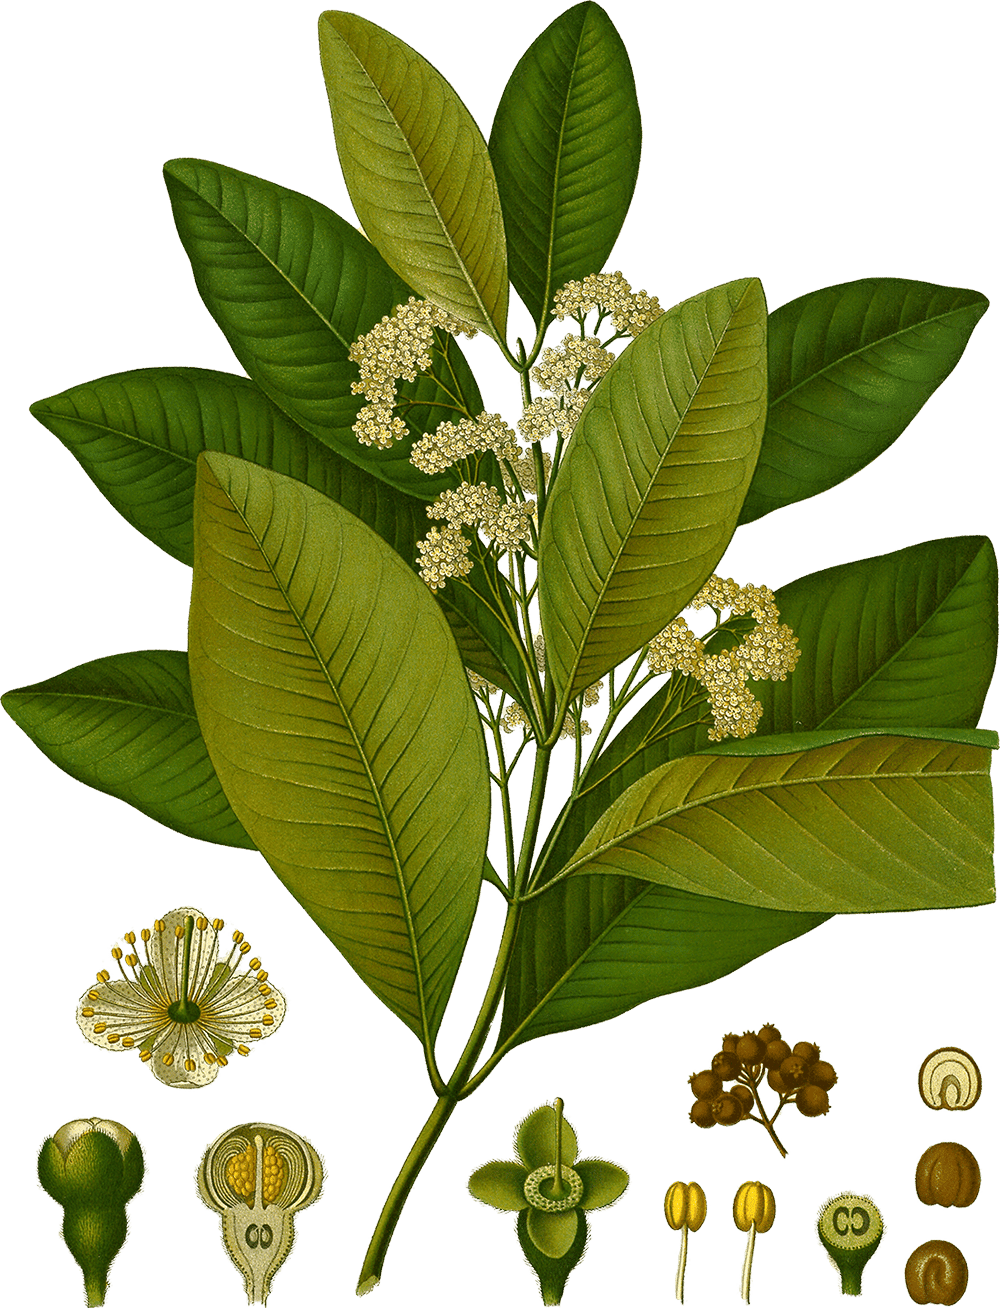
\includegraphics[width=0.25\textwidth]{imgs/kohler/allspice_kohler_min.png}
%   \caption{Allspice}
% \end{wrapfigure}

% The \gls{latex} typesetting markup language is specially suitable 
% for documents that are annoying to make.

% Glossaries like the above have to be set in the glossary.tex, and then called:
% This is the first time \gls{POWO} appears, and the second time \gls{POWO} appears. For plural and capital varieties:
% \gls{cultigen} and \glspl{cultigen}; \Gls{taxon} and \Glspl{taxon}

% \bigskip

% The index one\index{one} is here and two\index{two} is here. There is also index for tables \index{three|tb}, figures\index{four|fg}, and footnotes\index{five|fn}.
% Also, there is grouped indexing possible for things like black pepper\index{pepper!black}, white pepper\index{pepper!white}, and green pepper\index{pepper!green}. 

% WARNING: The index on Overleaf only prints on your pdf if you run it for the first time/clear the cache. I don't know why, currently unsolved.

% \section{Citations}

% Citation examples, such as \autocite[99]{huang_routledge_2019} and \textcite{huang_routledge_2019}. 
% Multi-volume citing also available, \pvolcite[]{9}[99]{bearman_encyclopaedia_1960} \& \tvolcite[]{9}[99]{bearman_encyclopaedia_1960}.

% \section{Environments}

% \begin{note}
%     This is a note.
% \end{note}

% \begin{equation}
%     \label{eq:1}
%     x^2  = 1
% \end{equation}

% And this was an equation. In Equation \ref{eq:1} we have~$\sqrt{\log n}$.

% \ex
% \begingl
% \gla\rightcomment{Hungarian (Finno-Ugric, \emph{reference})}Ez egy példám.//
% \glb This a example.my//
% \glft ``This is an example of mine.''//
% \endgl
% \xe




% \begin{etymology}\label{etym:pepper}
% \raggedright
% English \textit{pepper}
% < Middle English \textit{peper}
% < Old English \textit{pipor}
% < West Germanic \textit{*piper}
% < Latin \textit{piper} `black pepper, long pepper'
% < Ancient Greek \textit{péperi} `pepper'
% < Pahlavi
% < Middle Indo-Aryan \textit{pipparī} `long pepper'
% < Sanskrit \textit{pippalī} `berry, peppercorn', \textit{pippali} `long pepper'
% \end{etymology}

% \begin{spice}
% \textsc{Black pepper} \hfill \href{https://powo.science.kew.org/taxon/682369-1}{POWO} \\ 
% \textbf{English:} \textit{pepper; black pepper}. \textbf{Hungarian:} \textit{bors, fekete bors}. \textbf{Arabic:} فلفل، فلفل أسود \textit{filfil/fulful, filfil/fulful aswad}. \textbf{Chinese:} 胡椒, 黑胡椒 \textit{hújiāo, hēihújiāo} [nan]. \\
% \noindent{\color{black}\rule[0.5ex]{\linewidth}{.5pt}}
% \vspace*{-2.5\multicolsep}
% \begin{multicols}{2}
% \begin{tabular}{@{}ll@{}}
% Plant species: & \textit{Piper nigrum L.} \\
% Family: & \textit{Piperaceae} \\
% Region of oigin: & South India \\
% Plant part(s) used: & fruit; unripe fruit \\
% Color: & black; white; green \\
% \end{tabular}
% \end{multicols}
% \end{spice}

% This is a ref for Etymology \ref{etym:pepper} and then this is a cleverref for \Cref{sec:test}.

% \blindtext

% \poemtitle{Un poem de la lalala}
% \settowidth{\versewidth}{Fallait-il que je ecteffst vous aimasse,}
% \begin{verse}[\versewidth]
%  Fallait-il que je ecteffst vous aimasse, \\
%  Que vous me désespérassiez, \\
%  Et qu’en vain je m’opiniâtrasse, \\
%  Et que je vous idolâtrasse \\
%  Pour que vous m’a\lgSS a\lgSS ina\lgSS iez ! \\
% \end{verse}
% \attrib{Je ne sai qui}

% \begin{quote}
% \textsc{``Another remedy which the Goddess Isis prepared for the God Ra to drive out the pains that are in his head!}

% \smallskip
% Berry-of-the-Coriander---I\\
% Berry-of-the-Poppy-plant---I\\
% Wormwood---I\\
% Berry-of-the-sames-plant---I\\
% Berry-of-the-Juniper-plant---I\\
% Honey---I
% \smallskip

% Make into one, mix with Honey, and smear therewith in order to make him well forthwith. When this remedy is used by him against all illnesses in the head and all sufferings and evils of any sort, he will instantly become well.'' \textcite[40]{bryan_papyrus_1930}
% \end{quote}

% \begin{figure}[!hbt]
%     \centering
%     \subfloat{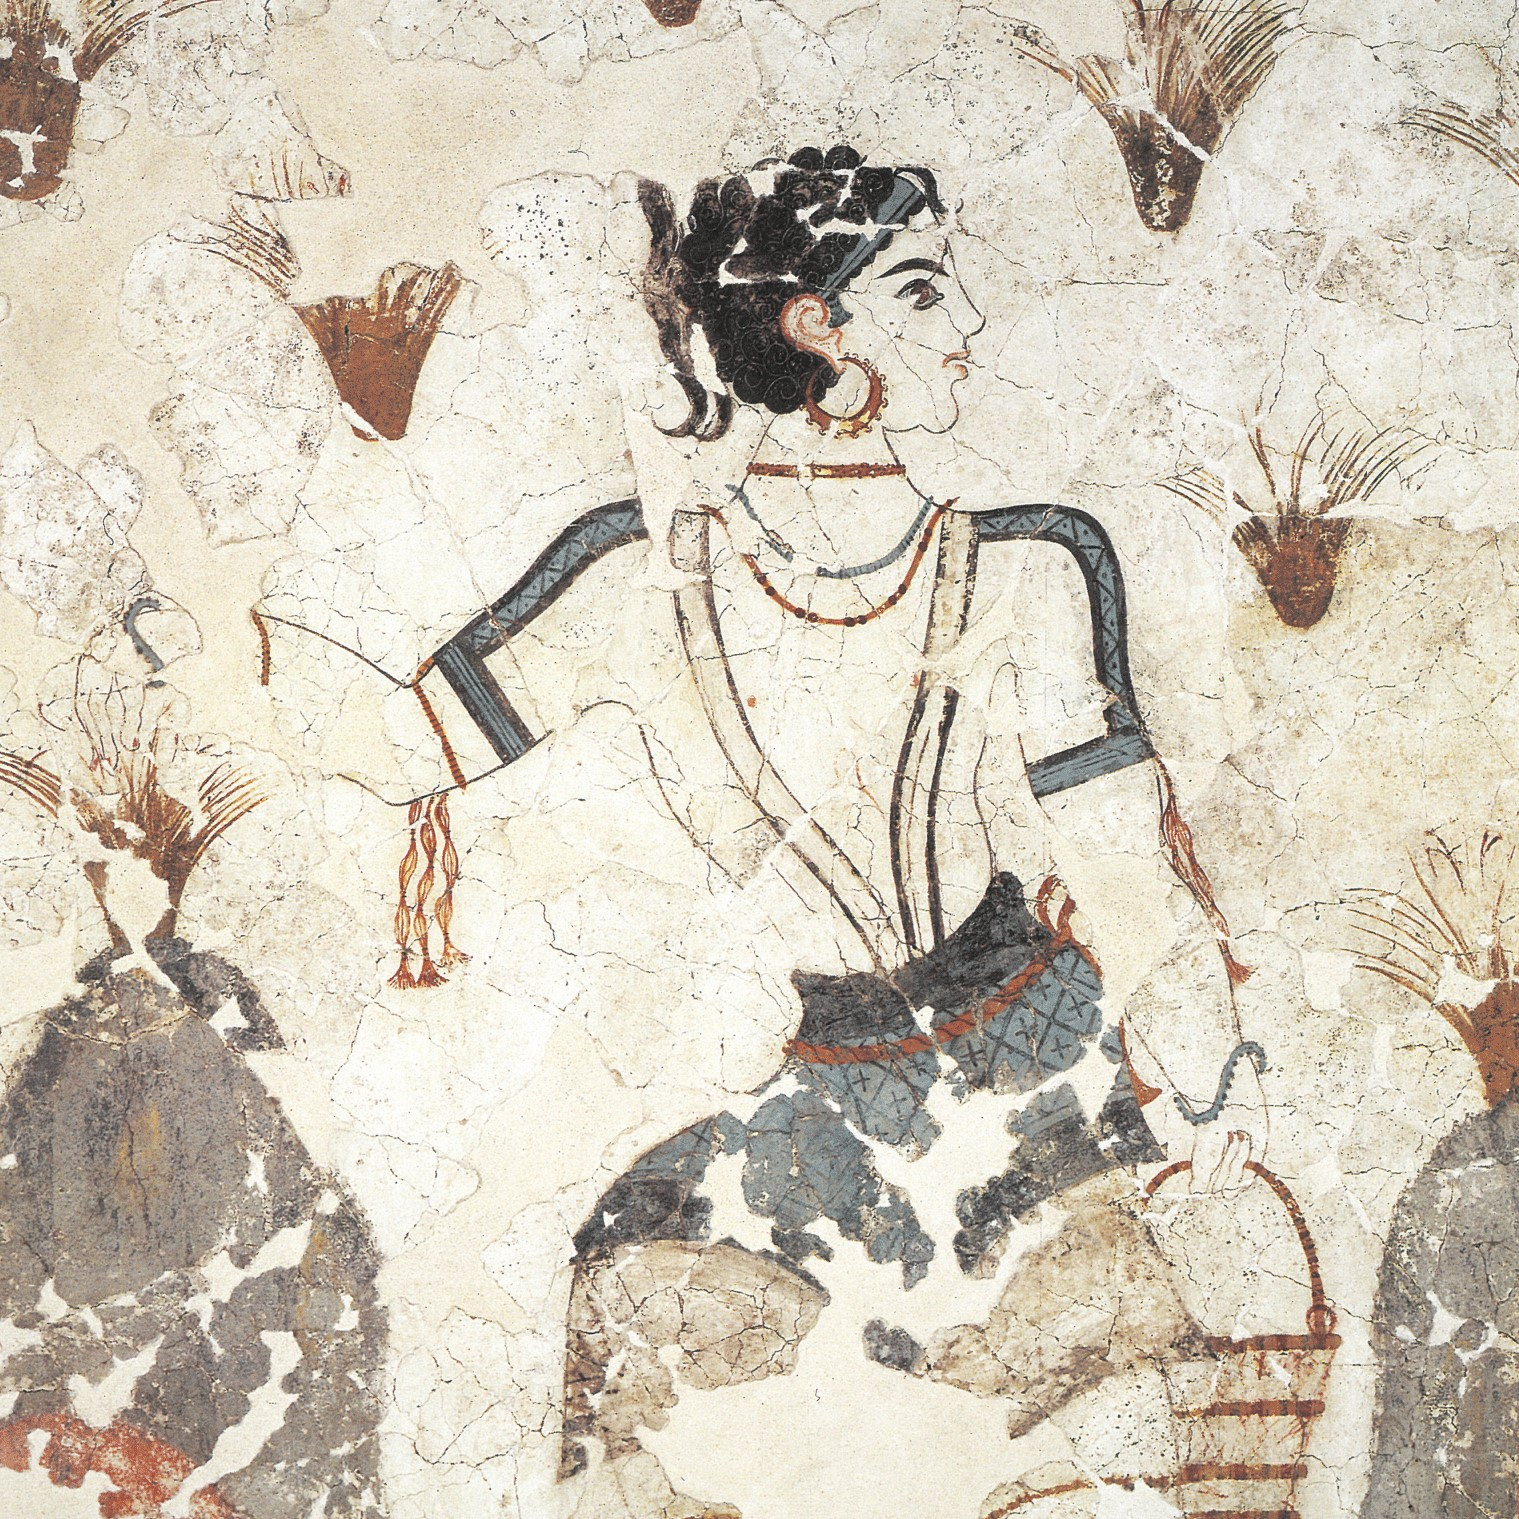
\includegraphics[width=0.482\linewidth]{imgs/saffron_gatherers_l.jpg}}
%     \hfill
%     \subfloat{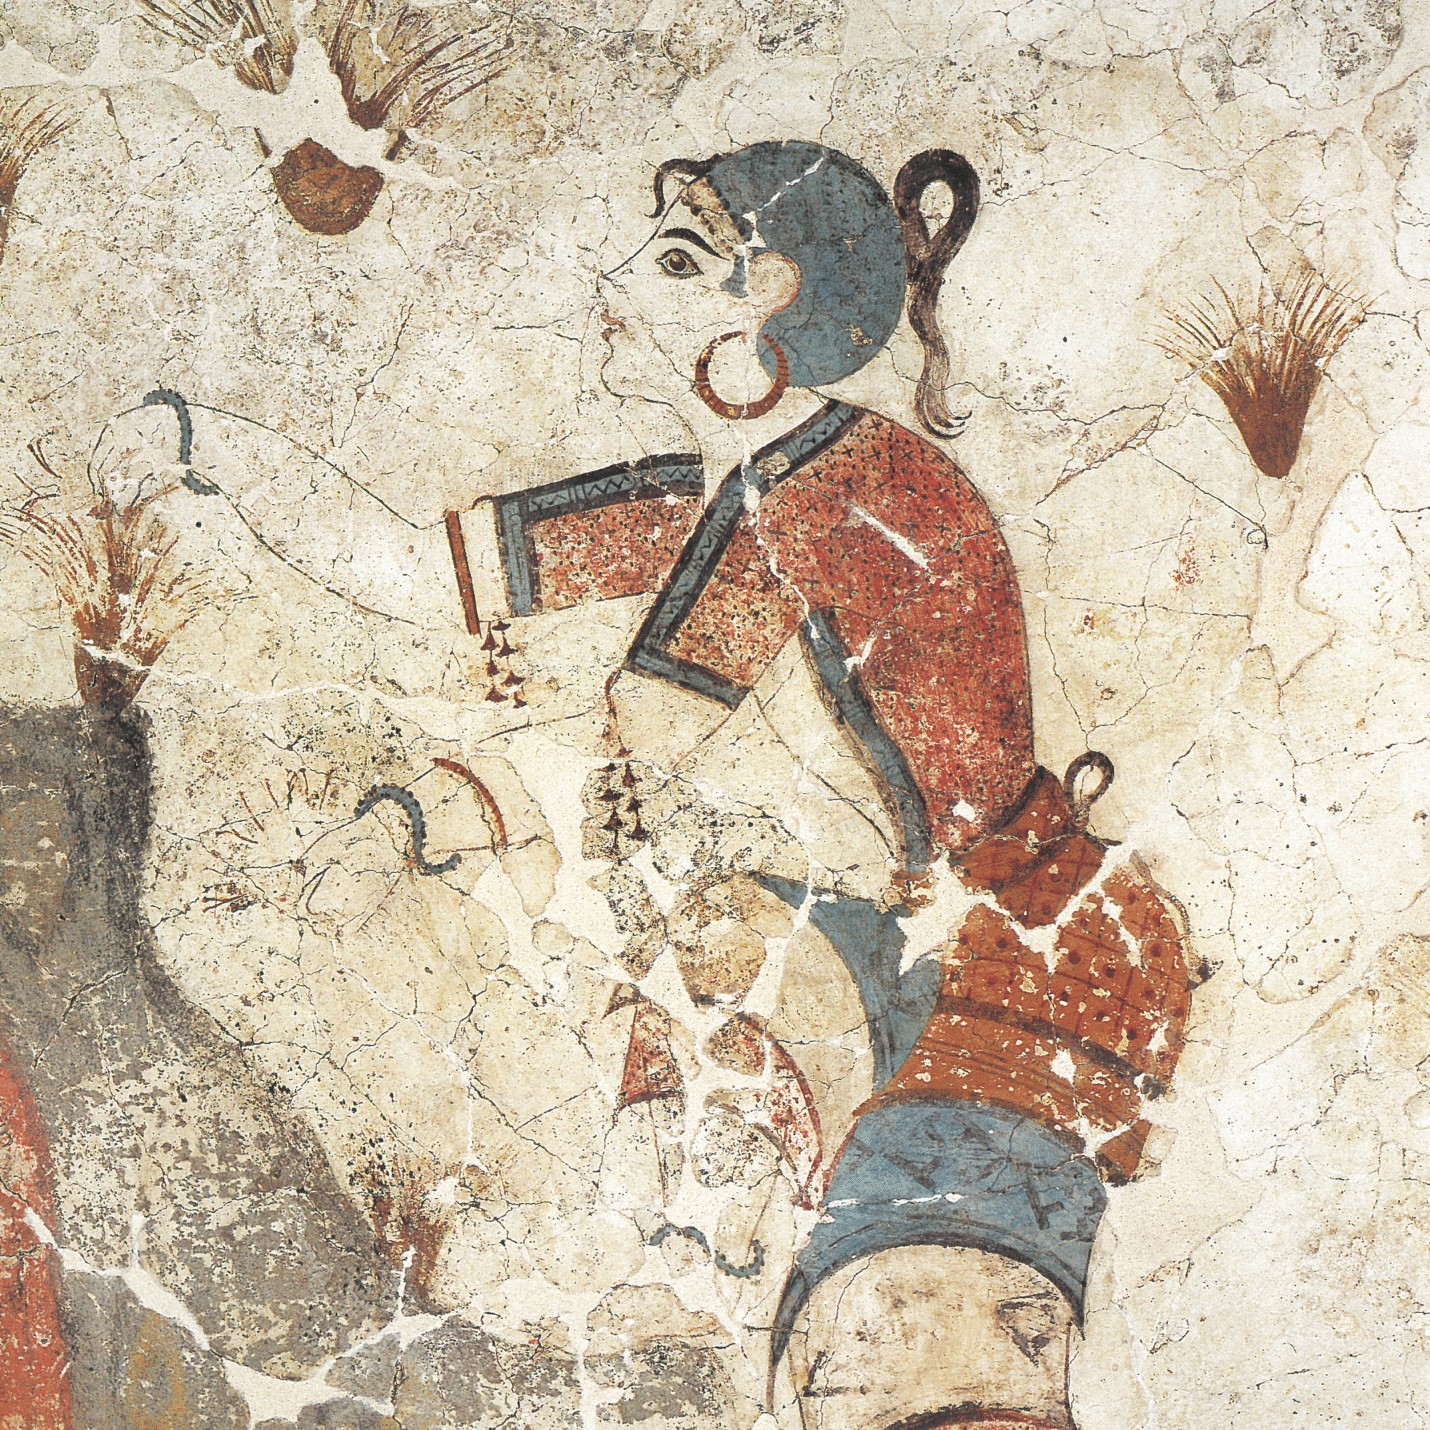
\includegraphics[width=0.482\linewidth]{imgs/saffron_gatherers_r.jpg}}
%     \caption{Saffron-gatherers. Details from the mural on the east wall in room 3a, first floor, at Xeste 3 site, Akrotiri at Thera \autocite[152]{doumas_wall-paintings_1992}.}
%     \label{fig:saffron_gatherers}
% \end{figure}

% \epigraph{By convention sweet and by convention bitter, by convention hot, by convention cold, by convention color; but in reality atoms and void.}{Democritus, \nth{3} century BC\\(DK 68B9, trans. Taylor 1999a)}

% % \epigraph{We shall not cease from exploration. And the end of all our exploring. Will be to arrive where we started. And know the place for the first time.}{T. S. Eliot}

% \section{IPA}

% \textipa{[ðIsIzsAmaIpeI]}, \textipa{[Its\*rilijizitutaIp]} as in: ``This is some IPA, it's really easy to type.''

% \begin{longtable}{p{0.15\textwidth}p{0.3\textwidth}p{0.3\textwidth}}
%   \toprule
%   \endfirsthead
%   \toprule
%   \endhead
%   \bottomrule
%   \endfoot
%   \bottomrule
%   \endlastfoot
%   Consonant & Onset & Coda\tabularnewline

%   \midrule p & pun.za (claw) & \textipa{k\super hap.Ra} (old man)\tabularnewline

%   b & \textipa{bO\|[d\super h} (bull) & \textipa{Seb.Ra} (dull)\tabularnewline

%   \textipa{b\super h} & \textipa{b\super he\:d} (sheep) & \tabularnewline

%   m & \textipa{mE} (me) & \textipa{amb} (mango)\tabularnewline

%   f & ful (flower) & \tabularnewline

%   \textipa{V} & \textipa{Vi\|[d.jaR.\|[t\super hi} & \textipa{RoVa}
%   (injury)\tabularnewline

%   \textipa{\|[t} & \textipa{\|[tu} (you) & \textipa{mO\|[t}
%   (don't)\tabularnewline

%   \textipa{\|[d} & \textipa{\|[deS} (many) & \textipa{swa\|[d}\tabularnewline

%   \textipa{\|[t\super h} & \textipa{\|[t\super he\:n.\:di} (cold) &
%   \textipa{hO\|[t\super h} (hand)\tabularnewline

%   \textipa{\|[d\super h} & \textipa{\|[d\super hus.ki} (down) &
%   \textipa{bO\|[d\super h} (bull)\tabularnewline

%   \textipa{\t*{ts}} & \textipa{\t*{ts}Ol.\:na} (to walk) & \textipa{so\t*{ts}}
%   (think)\tabularnewline

%   \textipa{\t*{ts}\super h} & \textipa{\t*{ts}\super hekke} (fast) &
%   \tabularnewline

%   \textipa{\t*{dz}} & \textipa{\t*{dz}a.\:na} (to go) & \tabularnewline

%   \textipa{n} & \textipa{n@i} (no) & \textipa{an.\|[dRe} (inside)\tabularnewline

%   \textipa{R} & \textipa{me.Ri} (my) & \textipa{g\super hOR}\tabularnewline

%   \textipa{s} & \textipa{sen.\|[tRi} (orange colour) & \textipa{hOs\:na} (to
%   laugh)\tabularnewline

%   \textipa{z} & \textipa{ze\:d} (root) & \textipa{Roz} (everyday)\tabularnewline

%   \textipa{l} & \textipa{lOm.ma} (long) & \textipa{kal}
%   (yesterday)\tabularnewline

%   \textipa{S} & \textipa{Sob.la} (beautiful) & \textipa{gaS}
%   (rain)\tabularnewline

%   \textipa{\:t} & \textipa{\:te\:d.\:da} (curved) & \textipa{nO\:t.\:t\super he}
%   (gone)\tabularnewline

%   \textipa{\:t\super h} & \textipa{\:t\super he\:n\:ra} (cold) &
%   \textipa{nO\:t.\:t\super he} (gone)\tabularnewline

%   \textipa{\:d} & & \textipa{ne\:d} (near)\tabularnewline

%   \textipa{\:d\super h} & & \textipa{pO\:d\super h.na} (to read)\tabularnewline

%   \textipa{\:r} & \textipa{pO\:ru} (fell) & \textipa{me\:n.\:r\super h@k}
%   (frog)\tabularnewline

%   \textipa{\:n} & \textipa{\|[de.\:na} (to give) & \textipa{ku\:n}
%   (who)\tabularnewline

%   \textipa{\:l} & \textipa{ke\:la} (banana) & \tabularnewline

%   \textipa{\t*{tS}} & \textipa{\t*{tS}Ok.ku\|[da} (rotten) & \tabularnewline

%   \textipa{\t*{dZ}} & \textipa{\t*{dZ}epuR} (Jaipur) & \tabularnewline

%   \textipa{j} & \textipa{ja\|[d} (remember) & \textipa{gaj}
%   (abuse)\tabularnewline

%   \textipa{k} & \textipa{ki.\:ra} (snake) & \textipa{b\super huk}
%   (hunger)\tabularnewline

%   \textipa{g} & \textipa{ga} (cow) & \textipa{b\super hEg.\:na} (to
%   run)\tabularnewline

%   \textipa{k\super h} & \textipa{k\super ha\:na} (to eat) & \textipa{paNk\super
%     h} (wing)\tabularnewline

%   \textipa{g\super h} & \textipa{g\super hOR} (house) & \tabularnewline

% \end{longtable}


% \section{Notes}

% A thesis submitted for examination purpose should include the words ‘Initial Submission for Examination Purpose’ lettered on the front cover. For details, see: this link \url{https://www.polyu.edu.hk/gs/rpghandbook/ref-regulations-format-thesis/} or the \href{https://www.polyu.edu.hk/gs/rpghandbook/section10/}{RPg Handbook}
% Transliteration of Arabic script: \href{https://referenceworks.brillonline.com/pages/help/transliteration-islam}{Brill Online}

% \epigraph{We shall not cease from exploration. And the end of all our exploring. Will be to arrive where we started. And know the place for the first time.}{T. S. Eliot}
% \index{epighraph}


% \epigraph{Maths is hell}{Tom, 2021}

% ⸙
% ♰ West Syriac cross
% 2671 ♱ East Syriac cross
% 2720 ✠ Maltese cross
% 2626 ☦ orthodox cross
% 2627 ☧ khi rho, Christogram
% 2628 ☨ cross of Lorraine
% 2629 ☩ cross of Jerusalem
% 2721 ✡ star of David
% 262A ☪ star and crescent
% 262B ☫ Farsi symbol
% 2638 ☸ wheel of dharma
% 262C ☬ ādi śakti or khaṇḍā
% 263D ☽ first quarter moon
% 263E ☾ last quarter moon
% \index[bot]{Cinnamomum verum}

% \blindtext

% \section{Ideas}

% Spices in the Bible

% Queen of Sheba in 1 Kings 10:25

% Story of Joseph 

% Make tree of who taught who in Hungarian orientalists.

% Shipnames and their origins: caravel, galleon, dhow, lateen, junk...

% Mapping Spice Words - A Linguistic Account of the Spice Trade

% Eating the Sinoshphere - Tracing gastronomical loanwords in East Asia

% 1873 Vienna

% Spice names as verbs: pepper, spice, bors, falfala

% Vanilla as boredom

% Chili pepper vs black pepper RED vs BLACK

% marcher d'un pas menu.
% se nettoyer la bouche, le dent.
% friser, boueler.

% berjalan dengan melagak, sombong

% contact induced similarities

% The (c. 3rd century) Nanzhou yiwu zhi (?????, "Record of Strange Things of the Southern Continent") or Nanfang yiwu zhi (?????, "Record of Strange Things of the South") was written by Wan Zhen (??), and may have been one of Ji Han's sources for his book. 

% Spice trade computer game 

% serendipity

% binomial name

% phytonym

% \section{Trees}

% \section{Example}

% best solution:

% \begin{forest}
%     for tree={align=center,calign=center}
%     [paprika\\{English},tier=a,baseline
%     [paprika\\{Hungarian},tier=b
%     [paprika\\{Serbian-Croatian-Bosnian},tier=c
%     [*pĭpĭrĭ\\{Proto-Slavic},tier=d
%     [piper\\{Latin},tier=e, before computing xy={s=-s("!u")},
%     [péperi\\{Ancient Greek},name=AG,tier=f, edge to=MG,
%     [?\\{Pahlavi},tier=g
%     [pipparī\\{Middle Indo-Aryan},tier=h
%     [pippalī\\{Sanskrit},tier=i]]]]]] 
%     [piperi\\{Modern Greek},name=MG]]]]
% \end{forest}

% \begin{forest}
%     for tree={align=center,calign=first}
%     [,l sep=0
%     [paprika\\\small{English},no edge,tier=a,baseline
%     [paprika\\\small{Hungarian},edge={line width=2pt},tier=b
%     [pàprika\\\small{Serbian-Croatian-Bosnian},tier=c
%     [*pĭpĭrĭ\\\small{Proto-Slavic},tier=d
%     [piper\\\small{Latin},tier=e
%     [péperi\\\small{Ancient Greek},name=AG,tier=f 
%     [?\\\small{Pahlavi},tier=g
%     [pipparī\\\small{Middle Indo-Aryan},tier=h
%     [pippalī\\\small{Sanskrit},tier=i]]]]]] 
%     [piperi\\\small{Modern Greek},edge=dashed,name=MG,edge label={node[midway,below,font=\scriptsize]{influenced}}]
%     ]]]
%     [1839,no edge,tier=a
%     [1569,no edge,tier=b
%     [c,no edge,tier=c
%     [d,no edge,tier=d
%     [e,no edge,tier=e
%     [f,no edge,tier=f
%     [g,no edge,tier=g
%     [h,no edge,tier=h
%     [i,no edge,tier=i]]]]]]]]]
%     [\href{https://www.etymonline.com/word/paprika\#etymonline_v_3108}{Etymonline},no edge,tier=a
%     [source,no edge,tier=b
%     [source,no edge,tier=c
%     [source,no edge,tier=d
%     [source,no edge,tier=e
%     [source,no edge,tier=f
%     [source,no edge,tier=g
%     [source,no edge,tier=h
%     [source,no edge,tier=i]]]]]]]]]
%     ]  
%     \draw[-] (AG.north) to node[above] {\scriptsize{a}} node[below] {\scriptsize{b}} (MG.south);
%     \draw[->,dotted] (AG) to[out=east,in=south] (MG);
% \end{forest}

% \begin{tabular}[t]{ll@{}}
% \tikz[baseline]\draw(0,1ex)--(1,1ex); & borrowed\\
% \tikz[baseline]\draw[dotted](0,1ex)--(1,1ex); & descended\\
% \tikz[baseline]\draw[dashed](0,1ex)--(1,1ex); & influenced\\
% \end{tabular}


% \begin{folio}{Stuff}\label{folio:pepper}
%     \begin{forest}
%         for tree={align=center,calign=first}
%         [,l sep=0
%         [paprika\\\small{English},no edge,tier=a,baseline
%         [paprika\\\small{Hungarian},edge={line width=2pt},tier=b
%         [pàprika\\\small{Serbian-Croatian-Bosnian},tier=c
%         [*pĭpĭrĭ\\\small{Proto-Slavic},tier=d
%         [piper\\\small{Latin},tier=e
%         [péperi\\\small{Ancient Greek},name=AG,tier=f 
%         [?\\\small{Pahlavi},tier=g
%         [pipparī\\\small{Middle Indo-Aryan},tier=h
%         [pippalī\\\small{Sanskrit},tier=i]]]]]] 
%         [piperi\\\small{Modern Greek},edge=dashed,name=MG,edge label={node[midway,below,font=\scriptsize]{influenced}}]]]]
%         [1839,no edge,tier=a
%         [1569,no edge,tier=b
%         [c,no edge,tier=c
%         [d,no edge,tier=d
%         [e,no edge,tier=e
%         [f,no edge,tier=f
%         [g,no edge,tier=g
%         [h,no edge,tier=h
%         [i,no edge,tier=i]]]]]]]]]
%         [\href{https://www.etymonline.com/word/paprika\#etymonline_v_3108}{Etymonline},no edge,tier=a
%         [source,no edge,tier=b
%         [source,no edge,tier=c
%         [source,no edge,tier=d
%         [source,no edge,tier=e
%         [source,no edge,tier=f
%         [source,no edge,tier=g
%         [source,no edge,tier=h
%         [source,no edge,tier=i]]]]]]]]]
%         ]  
%         \draw[-] (AG.north) to node[above] {\scriptsize{a}} node[below] {\scriptsize{b}} (MG.south);
%         \draw[->,dotted] (AG) to[out=east,in=south] (MG);
%     \end{forest}
%     \hfill
%     \begin{tabular}[t]{ll@{}}
%         \tikz[baseline]\draw(0,1ex)--(1,1ex); & borrowed\\
%         \tikz[baseline]\draw[dotted](0,1ex)--(1,1ex); & descended\\
%         \tikz[baseline]\draw[dashed](0,1ex)--(1,1ex); & influenced\\
%     \end{tabular}
% \end{folio}

% This last page is Folio \ref{folio:pepper}.

% \section{Example}

% \begin{forest}
%     for tree={align=center,calign=first}
%     [,l sep=0
%     [paprika\\\small{English},no edge,tier=a,baseline
%     [paprika\\\small{Hungarian},edge={line width=2pt},tier=b
%     [pàprika\\\small{Serbian-Croatian-Bosnian},tier=c
%     [*pĭpĭrĭ\\\small{Proto-Slavic},tier=d
%     [piper\\\small{Latin},tier=e
%     [péperi\\\small{Ancient Greek},name=AG,tier=f 
%     [?\\\small{Pahlavi},tier=g
%     [pipparī\\\small{Middle Indo-Aryan},tier=h
%     [pippalī\\\small{Sanskrit},tier=i]]]]]] 
%     [piperi\\\small{Modern Greek},edge=dashed,name=MG,edge label={node[midway,below,font=\scriptsize]{influenced}}]
%     ]]]
%     [1839,no edge,tier=a
%     [1569,no edge,tier=b
%     [c,no edge,tier=c
%     [d,no edge,tier=d
%     [e,no edge,tier=e
%     [f,no edge,tier=f
%     [g,no edge,tier=g
%     [h,no edge,tier=h
%     [i,no edge,tier=i]]]]]]]]]
%     [\href{https://www.etymonline.com/word/paprika\#etymonline_v_3108}{Etymonline},no edge,tier=a
%     [source,no edge,tier=b
%     [source,no edge,tier=c
%     [source,no edge,tier=d
%     [source,no edge,tier=e
%     [source,no edge,tier=f
%     [source,no edge,tier=g
%     [source,no edge,tier=h
%     [source,no edge,tier=i]]]]]]]]]
%     ]  
%     \draw[-] (AG.north) to node[above] {\scriptsize{a}} node[below] {\scriptsize{b}} (MG.south);
%     \draw[->,dotted] (AG) to[out=east,in=south] (MG);
% \end{forest}

% \begin{tabular}[t]{ll@{}}
% \tikz[baseline]\draw(0,1ex)--(1,1ex); & borrowed\\
% \tikz[baseline]\draw[dotted](0,1ex)--(1,1ex); & descended\\
% \tikz[baseline]\draw[dashed](0,1ex)--(1,1ex); & influenced\\
% \end{tabular}

% or

% \begin{forest}
%     for tree={align=center}
%     [paprika\\\small{English}
%     [paprika\\\small{Hungarian} 
%     [pàprika\\\small{Serbian-Croatian-Bosnian} 
%     [*pĭpĭrĭ\\\small{Proto-Slavic} 
%     [piper\\\small{Latin} 
%     [péperi\\\small{Ancient Greek},name=AG 
%     [*\\\small{Pahlavi} 
%     [pipparī\\\small{Middle Indo-Aryan} 
%     [pippalī\\\small{Sanskrit}]]]]]] 
%     [piperi\\\small{Modern Greek},edge=dashed,name=MG]]]]
%     \draw[-] (AG.north) to (MG.south);
%     \draw[->,dotted] (AG) to[out=east,in=south] (MG);
% \end{forest}

